\documentclass[conference]{IEEEtran}
\IEEEoverridecommandlockouts
% The preceding line is only needed to identify funding in the first footnote. If that is unneeded, please comment it out.
\usepackage{cite}
\usepackage{amsmath,amssymb,amsfonts}
\usepackage{algorithmic}
\usepackage{graphicx}
\usepackage{textcomp}
\usepackage{xcolor}
\def\BibTeX{{\rm B\kern-.05em{\sc i\kern-.025em b}\kern-.08em
    T\kern-.1667em\lower.7ex\hbox{E}\kern-.125emX}}
\begin{document}

\title{Towards a Transfer Learning Approach from Attention Based Synthetic ECG Analysis}
% {\footnotesize \textsuperscript{*}Note: Sub-titles are not captured in Xplore and
% should not be used}
% \thanks{Identify applicable funding agency here. If none, delete this
% }
\author{
\IEEEauthorblockN{K. A. Ishan Fernando}
\IEEEauthorblockA{\textit{Department of Computer Engineering} \\
\textit{University of Peradeniya}\\
Peradeniya, Sri Lanka \\
e18098@eng.pdn.ac.lk}\and
\and
\IEEEauthorblockN{K. N. Adeepa Fernando}
\IEEEauthorblockA{\textit{Department of Computer Engineering} \\
\textit{University of Peradeniya}\\
Peradeniya, Sri Lanka \\
e18100@eng.pdn.ac.lk}\and
\and
\IEEEauthorblockN{J. W. K. Ridma B. Jayasundara}
\IEEEauthorblockA{\textit{Department of Computer Engineering} \\
\textit{University of Peradeniya}\\
Peradeniya, Sri Lanka \\
e18155@eng.pdn.ac.lk}\and
\and
\IEEEauthorblockN{Prof. Roshan G. Ragel}
\IEEEauthorblockA{\textit{Department of Computer Engineering} \\
\textit{University of Peradeniya}\\
Peradeniya, Sri Lanka \\
roshanr@eng.pdn.ac.lk}\and
\and
\IEEEauthorblockN{Prof. Vajira Thambawita}
\IEEEauthorblockA{\textit{Department of Holistic Systems} \\
% ########### IF WE ADD THE FULL NAME HERE. THE FORMATIING CHANGES
\textit{Simula Metropolitan Center for }\\
\textit{Digital Engineering}\\
Norway \\
vajira@simula.no}\and
\and
\IEEEauthorblockN{Dr. Isuru Nawinne}
\IEEEauthorblockA{\textit{Department of Computer Engineering} \\
\textit{University of Peradeniya}\\
Peradeniya, Sri Lanka \\
isurunawinne@eng.pdn.ac.lk}\and
\and
}

\maketitle

\begin{abstract}
The leading cause of death in humans, Cardiovascular diseases\cite{b10} could be diagnosed by analysis of electrocardiogram (ECG) which is a non-invasive method that records electrical activity of the cardiac cycle. Due to the rise of privacy issues in using ECG records of patients for research purposes\cite{b1}, synthetic generated data with similar information and distribution have become an alternative. Attention based mechanism which is the basis of Transformer Neural Networks combined with other models such as Convolutional Neural Networks, Recurrent Neural Networks and Long-Short Term Memory have been used in ECG classification tasks using real patient ecg data with promising outcomes. But analysis of properties of ECG signals using attention based regression methods on synthetic data and transferring the learned parameters for fine tuning on limited real data is the interest area of this review article.

\end{abstract}

\begin{IEEEkeywords}
ECG, Deep Learning, Transfer Learning, Transformers
\end{IEEEkeywords}

\section{Introduction}
In recent years, the integration of machine learning techniques with electrocardiogram (ECG) data analysis has sparked significant interest and promise in the field of healthcare. The ability to accurately predict vital physiological parameters, such as heart rate, QT interval, and other cardiac metrics, directly from ECG waveforms holds immense potential for revolutionizing clinical practice. This paper aims to provide a comprehensive review of the advancements, challenges, and future directions in utilizing machine learning for ECG regression and classification tasks.

The electrocardiogram, a fundamental tool in cardiology, provides a graphical representation of the electrical activity of the heart over time. Traditionally, ECG interpretation has relied on manual analysis by skilled clinicians, which can be time-consuming and prone to subjectivity. However, with the advent of machine learning, automated analysis of ECG signals has become increasingly feasible, offering the promise of more efficient and accurate diagnosis and monitoring.

One of the primary objectives in ECG analysis is the prediction of essential cardiac parameters directly from ECG waveforms. These parameters include but are not limited to heart rate, QT interval, QRS duration, and ST segment changes. Accurate estimation of these metrics is crucial for diagnosing various cardiac conditions, assessing cardiovascular risk, and guiding treatment decisions. Machine learning models, particularly deep learning architectures, have shown remarkable success in learning complex patterns from ECG data and making accurate predictions of these parameters.

\begin{figure}[htbp]
\centering
{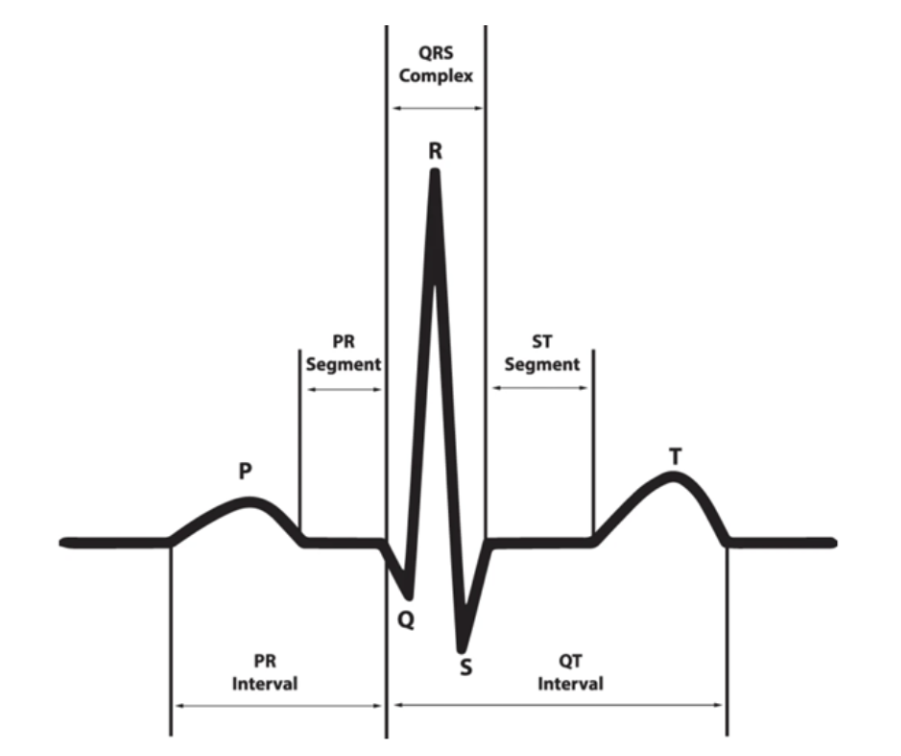
\includegraphics[scale=0.3]{fig1.png}}
\caption{ ECG \cite{b9}}
\label{fig}
\end{figure}

The electrocardiogram (ECG) shown in Figure 01 provides a visual representation of the heart's electrical activity, crucial for diagnosing various cardiac conditions. It features distinct waves – P, Q, R, S, and T – each indicative of different phases of the cardiac cycle. The P wave signifies atrial depolarization, initiating atrial contraction, while the QRS complex represents ventricular depolarization, essential for ventricular contraction. The T wave, on the other hand, signifies ventricular repolarization, preparing the heart for the next cycle. Moreover, the ECG delineates intervals and segments: the PR interval measures atrioventricular conduction time, the QT interval monitors ventricular depolarization and repolarization, the PR segment reflects AV nodal conduction, and the ST segment indicates early ventricular repolarization. Changes in these intervals and segments can signify abnormalities like arrhythmias, ischemic heart disease, or conduction disorders. Therefore, ECG analysis is pivotal in diagnosing and managing cardiovascular conditions, guiding treatment decisions and patient care effectively.

This review paper will delve into the diverse methodologies employed in leveraging machine learning for ECG regression and classification tasks. We will explore the different types of machine learning algorithms utilized, ranging from traditional regression models to state-of-the-art deep learning architectures such as convolutional neural networks (CNNs), recurrent neural networks (RNNs) and Vision Transformers (ViT). Additionally, we will discuss the challenges inherent in ECG regression and classification, including data quality issues, dataset heterogeneity, and interpretability of model predictions.

Furthermore, this paper will highlight the current applications and clinical implications of machine learning-based ECG regression. From early detection of arrhythmias to personalized risk stratification, the integration of machine learning into ECG analysis has the potential to transform patient care and improve outcomes.

Integrating machine learning with ECG data analysis marks a significant advancement in heart health. By harnessing the power of computers, we can enhance our comprehension of ECG results, enabling healthcare professionals to make more precise diagnoses and tailor treatments for patients effectively. This review delves into the transformative impact of this technology on cardiology, aiming to inspire further exploration and research in this vital field.


\section{Models}

Investigation of the use of machine learning models in ECG analysis, shows a number of previous studies applying deep learning methods that outperform traditional signal processing techniques\cite{b1}. Use of Residual CNN for classification of 6 types of abnormalities\cite{b2} using TNMG Brazil dataset, resulted in a high specificity of 99\%. 


\begin{equation}
\text{Specificity} = \frac{\text{True Negatives}}{\text{True Negatives} + \text{False Positives}}
\end{equation}

The EfficientNet CNN model used to diagnose multilabel abnormalities\cite{b3} has used ECG images from TNMG Brazil dataset with Grad-CAM for improved interpretability. Use of Echo State Network (ESN), a brain-inspired machine learning approach, for heart beat classification and arrhythmia detection\cite{b4} utilizes ensembles of ESNs \cite{b5} demonstrated high efficacy in achieving high accuracy while maintaining computational efficiency. 

A study\cite{b6} that ensembled  Support Vector Machine (SVM), k-Nearest Neighbors (kNN), Random Forest (RF) leveraging the MIT-BIH dataset Among the tested models, the Support Vector Machine (SVM) demonstrated the most promising performance. The paper\cite{b7} employed Logistic Regression (LR), Decision Tree (DT), Nearest Neighbor (NN), Naïve Bayes (NB), Support Vector Machine (SVM), and Artificial Neural Network (ANN) to predict the likelihood of certain heart diseases. The dataset was obtained from the UCI Machine Learning Repository. The Naïve Bayes resulted in 94\% accuracy for Coronary Artery Disease. 

Paper\cite{b8} published on classification of ECG signals, reviews a range of methodologies employed in previous studies, including Self Organizing Maps (SOM), Support Vector Machines (SVM), Multilayer Perceptron (MLP), Markov Models, and Fuzzy or Neuro-fuzzy Systems. However, the study opts for recurrent neural networks (RNNs) as the primary approach, specifically delving into different RNN architectures such as vanilla RNNs, gated recurrent units (GRUs), and long short-term memory (LSTM) networks. The results indicate that while various models have shown promise, LSTM networks outperform others, achieving an accuracy of 88.1\% in binary classification when employing three hidden layers with 64, 256, and 100 neurons respectively, and five iterations.

A research\cite{b11} employed deep learning architectures, specifically a 1D convolutional neural network (CNN), for the classification of electrocardiogram (ECG) data. The CNN architecture consisted of 7 convolutional layers with a filter width of 5 and 128 neurons, augmented with max-pooling and dropout layers after each convolutional layer, followed by a Global Average Pooling layer. The feature extraction phase was succeeded by 3 fully-connected layers with 256, 128, and 64 neurons respectively, each followed by dropout layers, culminating in a softmax layer with 4 outputs corresponding to the ECG classesThe model's performance was evaluated, demonstrating an accuracy of approximately 86\% on the validation dataset.

Another study for ECG detection with Deep Learning\cite{b12} accompanies CNN-based Deep Active Learning (DAL) model which produced an Entropy sampling accuracy = 98.99\%, Margin sampling accuracy = 98.99\%, Least confidence dropout = 99.02\% with the use of MIT-BIH dataset. Using SVM on the same dataset, the study\cite{b19} for multiclass detecting various arrhythmia types in ECG resulted in the accuracy for five classes as 97.48\%. In the two-stage SVM, accuracy for the normal class matched the single-stage SVM at 97.5\%, while true positive rates for arrhythmia classes improved or remained the same, leading to an average accuracy of 98.3%.

Since the introduction of the self-attention mechanism for Natural Language Processing (NLP) tasks, researches have shown interests in accompanying the very model for other areas including researches on ECG analysis and classification.


\begin{figure}[htbp]
\centering
{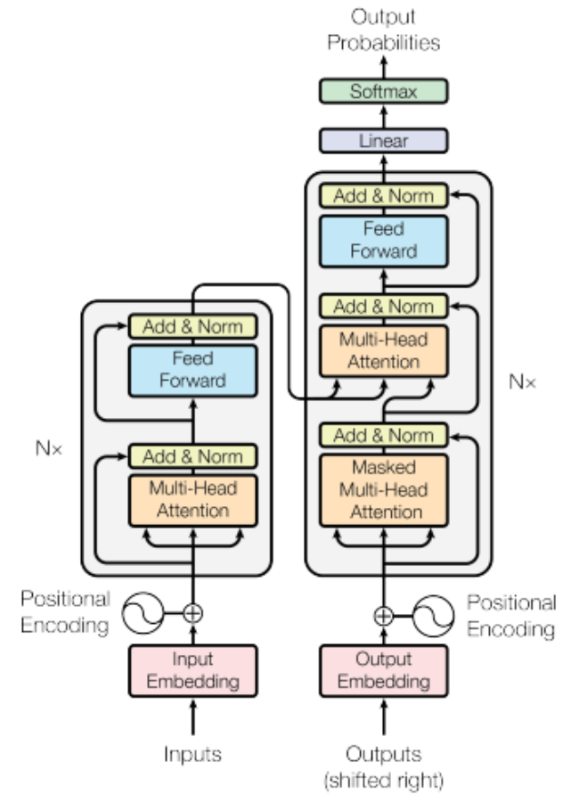
\includegraphics[scale=0.3]{fig2.png}}
\caption{Transformer Model Architecture \cite{b14}}
\label{fig}
\end{figure}

A study of ECG segmentation for detection of ECG beat parameters\cite{b15} uses an attention based Convolutional Bidirectional Long Short Term Memory (Conv-BiLSTM) with the advantage of BiLSTMs capturing temporal dependencies in the ECG signal \cite{b17}. The network leverages convolutional and bidirectional LSTM layers with self-attention mechanisms to capture local wave features and temporal context. Fiducial points like Pon, Poff, QRSon, etc., are then detected post-segmentation. With the use of PhysioNet’s QT database as the dataset, the achieved ECG segmentation accuracy was 95\% whereas fiducial point detection accuracy was 99.4%.
	
Another application with Wide and Deep Transformer Neural Network for 12-lead ECG classification\cite{b16} achieved the top score of 0.533 on the full dataset supplied for the 2020 PhysioNet/CinC challenge. . It combines static hand-crafted features with deep features extracted from raw ECG waveforms using convolution operations and a Transformer architecture. The Transformer's self-attention mechanism allows for faster training compared to traditional recurrent neural networks. Fully connected layers are then employed to combine wide and deep features for multi-label classification.

Use of ConvNeXt with Multimodal transformer\cite{b18} for ECG classification with the models Continuous Wavelet Transform (CWT), Improved ConvNeXt architecture, Multimodal Transformer Layer, Fused Multi-layer Perceptron (MLP) provides multiple high accuracy values with the use of same dataset MIT-BIH. Another study\cite{b20} developed ECT-net, combining CNN and transformer, to detect ECG waveforms by integrating local and global heart signal features, tested on the CPSC-DB. ECT-net achieved high F1 scores on P, QRS, and T waves, proving its effectiveness and generalization across various cardiac diseases.


\begin{equation}
    F1 = \frac{2*Precision*Recall}{Precision+Recall} = \frac{2*TP}{2*TP+FP+FN}
\end{equation}

A Heartbeat-aware Transformer model\cite{b21} for ECG analysis featuring a convolutional layer for initial processing, followed by an encoder-decoder structure with a unique heartbeat-aware attention mechanism was evaluated on a large ECG dataset from Yocaly, containing records from 200k patients, labeled for various arrhythmias. 

HeartBEiT\cite{b22}, a 12-layer transformer with 86M parameters, is compared to ImageNet's ViT-B/16 (86M), ResNet-152 (60M), and EfficientNet-B4 (19M) for ECG analysis .HeartBEiT outperformed CNN models (ViT-B/16, ResNet-152, EfficientNet-B4) in classifying low LVEF, diagnosing HCM, and detecting STEMI across varying training data sizes, with performance advantages more pronounced at lower data volumes and maintained superiority in external validations.The study utilized 8.5 million ECG records from Mount Sinai Health System and external PTB-XL dataset for model training and validation.	

A Vision Transformer with Deformable Attention\cite{b23} with the CNN-DVIT model outperformed ResNet, LSTM, and a competitor transformer-based model in ECG classification with an F1 score of 0.829. Its strong classification ability was evident, though some categories showed poorer performance due to limited data. AUC values exceeded 95\% for most classes on the ROC curve, except for ST-segment elevated. While another study with Vision Transformer in the form of ECG-Convolution-Vision Transformer Network ECVT-Net\cite{b24} inspired by both CNN and Vision transformer reached an accuracy of 98.88\% for the inter-patient scheme.



\section{Methods}

In the study\cite{b6}ECG signals underwent preprocessing steps, including normalization, denoising, and segmentation to extract relevant heartbeat segments. To optimize model performance, hyperparameter tuning was conducted using a HalvingGridSearchCV approach. Data Preprocessing\cite{b7} involved removal of null values, categorization into normal and abnormal ECG categories.Method involved train-test split (75-25), Fine Tuning: Cross-validation and random train-test split. Another study\cite{b12} started with pre-training on a small labeled dataset, then selects unlabeled samples for expert annotation. This process iterates until a target is met or no unlabeled samples remain, minimizing reliance on labeled data while ensuring high performance and quality annotations.

A study accompanying attention based model\cite{b15} preprocessing involves removing noise, standardizing signals, and applying wavelet transform. The preprocessing of another study with the use of ConvNeXt with Multimodal Transformer\cite{b18} included partitioning into 5-second segments with overlapping, denoising with DWT (Daubechies D6), resampling to 1280 sample points, and Z-score normalization. WPS preprocessing: noise and baseline drift removal, median filtering, wavelet transform denoising, segmentation into 5-second segments, resampling to 1280 sample points, and normalization.

The HearBeit\cite{b22} model used preprocessed ECGs into filtered images and trained models on predicting masked image parts using a Dall-E tokenizer for pre-training on unlabeled data. The ECVT-Net\cite{b24} used a pre-processing technique of resampling ECG to 250 Hz, segmenting around R point (0.4s before to 0.6s after),and  normalizing amplitude to [0,1], with layer normalization\cite{b25} done between layers.


\section{Limitations}


Machine learning models for ECG analysis have shown promising results but face significant limitations. Existing research lacks in evaluating the models' performance under noisy conditions, which is critical for real-world applications. Furthermore, while the novel CNN-ViT based models have achieved high accuracy, indicating its practical relevance, it still struggles with capturing long-term dependencies due to the limited receptive field size. This limitation is crucial for ECG signals, which, as 1D time series, require the extraction of correlations over different time periods for effective analysis. Despite the combined use of CNNs for local feature extraction and ViTs for mining global correlations, which enhances noise robustness, the challenge of accurately analyzing ECG signals under various noise levels and ensuring the capture of long-term dependencies remains a significant hurdle for these models.

Another noticeable limitation in the field of ECG analysis and classification is the scarcity of ECG data. The use of MIT-BIH dataset in most of the above reviewed researches \cite{b6},\cite{b12},\cite{b18} supports the fact that unavailability of ECG data in large amounts is due to privacy issues raised in sharing patient data\cite{b1}.



\section{Improvements}

Diagnosis of cardiovascular diseases through the analysis of ECG signals using Deep Learning algorithms always require continuous research due to the critical nature of the application and ability for improvement of performance metrics. Researches have progressed from baseline models to ensemble learning methods to increase the performances together with the efficiency of computation.

The study classifying ECG arrhythmias using LSTM networks\cite{b8} with high accuracy, highlights the potential for further exploration, such as integrating convolutional neural networks (CNNs) into the classification process for enhanced performance. In another research\cite{b11} involving 1D CNNs, despite achieving notable accuracy, the study acknowledges areas for potential improvement, such as exploring additional preprocessing techniques and employing Generative Adversarial Networks (GANs) to create a more balanced dataset, thereby suggesting avenues for enhancing the model's accuracy in future iterations.

Inorder to overcome the limitation of real ECG data, synthetic generated ECG data sets such as DeepFake ECG\cite{b1} could be used. Due to the requirement of high loads of data to train the Transformer model, using synthetic generated data and using Transfer Learning techniques to fine tune the parameters on limited real ECG data is the proposed approach in our review.

\begin{figure}[htbp]
\centering
{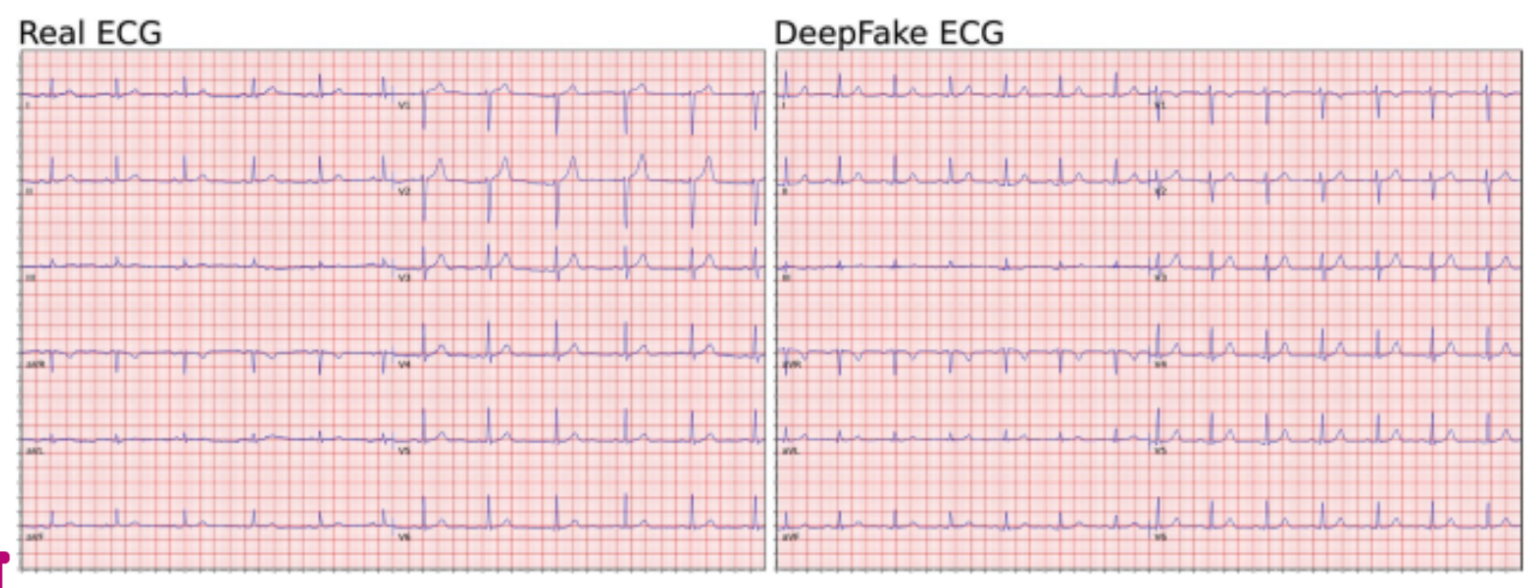
\includegraphics[scale=0.2]{fig3.png}}
\caption{ Real ECG (left lane) and a DeepFake ECG (right lane) \cite{b1}}
\label{fig}
\end{figure}

Due to the requirement of high loads of data to train the Transformer model, using synthetic generated data and using Transfer Learning techniques to fine tune the parameters on limited real ECG data is the proposed approach in our review.

\section{Conclusion}

In conclusion, this review paper thoroughly explores the integration of machine learning techniques for electrocardiogram (ECG) analysis, emphasizing the potential of deep learning models in revolutionizing clinical practice. The paper covers a wide range of models, including convolutional neural networks (CNNs), recurrent neural networks (RNNs), and Transformer-based architectures, showcasing their applications, strengths, and limitations in ECG regression and classification tasks.

The research focuses on the unique approach of utilizing synthetic ECG data, generated with attention-based mechanisms and Transformer Neural Networks, to address privacy concerns associated with real patient data. The attention-based regression methods on synthetic data, followed by fine-tuning on limited real data, present an innovative perspective in the field. This approach aims to overcome challenges related to data privacy and scarcity, making it a noteworthy contribution to the existing literature.

The paper recognizes the limitations of existing models, particularly their performance under noisy conditions and the struggle to capture long-term dependencies in ECG signals. The scarcity of large-scale ECG datasets, primarily due to privacy concerns, is also highlighted as a significant hurdle. To address these limitations, the paper suggests potential improvements, such as integrating additional preprocessing techniques, exploring GANs for data augmentation, and leveraging synthetic datasets like DeepFake ECG.

Throughout the review, the paper provides insights into the methodologies employed in previous studies, covering diverse machine learning models, their architectures, and preprocessing steps. The inclusion of real-world examples, such as the application of models on specific datasets and the achievement of high specificity in abnormality detection, adds practical relevance to the discussion.

In summary, this review paper contributes to the ongoing discourse in the field of ECG analysis and machine learning by presenting a comprehensive overview of existing models, addressing their limitations, proposing improvements, and introducing a novel approach using synthetic data for attention-based regression. It not only reviews the advancements made but also stimulates further exploration and research in this critical area, emphasizing the transformative impact of machine learning on cardiology and heart health.



\begin{thebibliography}{00}
\bibitem{b1}V. Thambawita et al., “DeepFake electrocardiograms using generative adversarial networks are the beginning of the end for privacy issues in medicine,” Scientific Reports, vol. 11, no. 1, Nov. 2021, doi: 10.1038/s41598-021-01295-2.
\bibitem{b2} A. H. Ribeiro et al., “Automatic diagnosis of the 12-lead ECG using a deep neural network,” Nature Communications, vol. 11, no. 1, Apr. 2020, doi: 10.1038/s41467-020-15432-4.

\bibitem{b3} V. Sangha et al., “Automated multilabel diagnosis on electrocardiographic images and signals,” Nature Communications, vol. 13, no. 1, Mar. 2022, doi: 10.1038/s41467-022-29153-3.

\bibitem{b4}  S. Aziz, S. Ahmed, and M.-S. Alouini, “ECG-based machine-learning algorithms for heartbeat classification,” Scientific Reports, vol. 11, no. 1, Sep. 2021, doi: 10.1038/s41598-021-97118-5.
\bibitem{b5} M. Javadi, R. Ebrahimpour, A. Sajedin, S. Faridi, and S. Zakernejad, “Improving ECG Classification Accuracy Using an Ensemble of Neural Network Modules,” PLoS ONE, vol. 6, no. 10, p. e24386, Oct. 2011, doi: 10.1371/journal.pone.0024386.

\bibitem{b6} M. Sraitih, Y. Jabrane, and A. Hajjam El Hassani, “An Automated System for ECG Arrhythmia Detection Using Machine Learning Techniques,” Journal of Clinical Medicine, vol. 10, no. 22, p. 5450, Nov. 2021, doi: 10.3390/jcm10225450.

\bibitem{b7} S. R. Tithi, A. Aktar, F. Aleem, and A. Chakrabarty, “ECG data analysis and heart disease prediction using machine learning algorithms,” 2019 IEEE Region 10 Symposium (TENSYMP), Jun. 2019, Published, doi: 10.1109/tensymp46218.2019.8971374.

\bibitem{b8}  S. Singh, S. K. Pandey, U. Pawar, and R. R. Janghel, “Classification of ECG Arrhythmia using Recurrent Neural Networks,” Procedia Computer Science, vol. 132, pp. 1290–1297, 2018, doi: 10.1016/j.procs.2018.05.045.

\bibitem{b9}  J. Zheng, J. Zhang, S. Danioko, H. Yao, H. Guo, and C. Rakovski, “A 12-lead electrocardiogram database for arrhythmia research covering more than 10,000 patients,” Scientific Data, vol. 7, no. 1, Feb. 2020, doi: 10.1038/s41597-020-0386-x.

\bibitem{b10} A. Natarajan et al., “A Wide and Deep Transformer Neural Network for 12-Lead ECG Classification,” 2020 Computing in Cardiology Conference (CinC), Dec. 2020, Published, doi: 10.22489/cinc.2020.107.

\bibitem{b11} B. Pyakillya, N. Kazachenko, and N. Mikhailovsky, “Deep Learning for ECG Classification,” Journal of Physics: Conference Series, vol. 913, p. 012004, Oct. 2017, doi: 10.1088/1742-6596/913/1/012004.

\bibitem{b12} H. Wang, Y. Zhou, B. Zhou, and Z. Wang, “A Novel Method for Detection of ECG with Deep Learning,” 2021 7th International Conference on Computer and Communications (ICCC), Dec. 2021, Published, doi: 10.1109/iccc54389.2021.9674506.

% \bibitem{b13} M. S. Haleem and L. Pecchia, “A Deep Learning Based ECG Segmentation Tool for Detection of ECG Beat Parameters,” 2022 IEEE Symposium on Computers and Communications (ISCC), Jun. 2022, Published, doi: 10.1109/iscc55528.2022.9912906.

\bibitem{b14}  C. Subakan, M. Ravanelli, S. Cornell, M. Bronzi, and J. Zhong, “Attention Is All You Need In Speech Separation,” ICASSP 2021 - 2021 IEEE International Conference on Acoustics, Speech and Signal Processing (ICASSP), Jun. 2021, Published, doi: 10.1109/icassp39728.2021.9413901.

\bibitem{b15} M. S. Haleem and L. Pecchia, “A Deep Learning Based ECG Segmentation Tool for Detection of ECG Beat Parameters,” 2022 IEEE Symposium on Computers and Communications (ISCC), Jun. 2022, Published, doi: 10.1109/iscc55528.2022.9912906.

\bibitem{b16} A. Natarajan et al., “A Wide and Deep Transformer Neural Network for 12-Lead ECG Classification,” 2020 Computing in Cardiology Conference (CinC), Dec. 2020, Published, doi: 10.22489/cinc.2020.107.

\bibitem{b17} X. Xu, S. Jeong, and J. Li, “Interpretation of Electrocardiogram (ECG) Rhythm by Combined CNN and BiLSTM,” IEEE Access, vol. 8, pp. 125380–125388, 2020, doi: 10.1109/access.2020.3006707.

\bibitem{b18} J. Zhu et al., “An Improved ConvNeXt with Multimodal Transformer for Physiological Signal Classification,” IEEE Access, pp. 1–1, 2024, doi: 10.1109/access.2024.3355273. 

\bibitem{b19} A. Singh and A. Kaul, "Analysis of ECG Signal using Machine Learning Approaches for Detecting different Heart Abnormalities," 2022 2nd International Conference on Emerging Frontiers in Electrical and Electronic Technologies (ICEFEET), Patna, India, 2022, pp. 1-5, doi: 10.1109/ICEFEET51821.2022.9848279

\bibitem{b20} D. Wang et al., “Inter-patient ECG characteristic wave detection based on convolutional neural network combined with transformer,” Biomedical Signal Processing and Control, vol. 81, p. 104436, Mar. 2023, doi: 10.1016/j.bspc.2022.104436.

\bibitem{b21} B. Wang, C. Liu, C. Hu, X. Liu, and J. Cao, “Arrhythmia Classification with Heartbeat-Aware Transformer,” ICASSP 2021 - 2021 IEEE International Conference on Acoustics, Speech and Signal Processing (ICASSP), Jun. 2021, Published, doi: 10.1109/icassp39728.2021.9413938.

\bibitem{b22} A. Vaid et al., “A foundational vision transformer improves diagnostic performance for electrocardiograms,” npj Digital Medicine, vol. 6, no. 1, Jun. 2023, doi: 10.1038/s41746-023-00840-9.

\bibitem{b23} Y. Dong, M. Zhang, L. Qiu, L. Wang, and Y. Yu, “An Arrhythmia Classification Model Based on Vision Transformer with Deformable Attention,” Micromachines, May 30, 2023. https://doi.org/10.3390/mi14061155 

\bibitem{b24} T. Liu et al., “Inter-Patient Congestive Heart Failure Detection Using ECG-Convolution-Vision Transformer Network,” Sensors, Apr. 25, 2022. https://doi.org/10.3390/s22093283  

\bibitem{b25} J. L. Ba, “Layer Normalization,” arXiv.org, Jul. 21, 2016. https://doi.org/10.48550/arXiv.1607.06450 

\end{thebibliography}


% %########################################################## template
% \section{Prepare Your Paper Before Styling}
% Before you begin to format your paper, first write and save the content as a 
% separate text file. Complete all content and organizational editing before 
% formatting. Please note sections \ref{AA}--\ref{SCM} below for more information on 
% proofreading, spelling and grammar.

% Keep your text and graphic files separate until after the text has been 
% formatted and styled. Do not number text heads---{\LaTeX} will do that 
% for you.

% \subsection{Abbreviations and Acronyms}\label{AA}
% Define abbreviations and acronyms the first time they are used in the text, 
% even after they have been defined in the abstract. Abbreviations such as 
% IEEE, SI, MKS, CGS, ac, dc, and rms do not have to be defined. Do not use 
% abbreviations in the title or heads unless they are unavoidable.

% \subsection{Units}
% \begin{itemize}
% \item Use either SI (MKS) or CGS as primary units. (SI units are encouraged.) English units may be used as secondary units (in parentheses). An exception would be the use of English units as identifiers in trade, such as ``3.5-inch disk drive''.
% \item Avoid combining SI and CGS units, such as current in amperes and magnetic field in oersteds. This often leads to confusion because equations do not balance dimensionally. If you must use mixed units, clearly state the units for each quantity that you use in an equation.
% \item Do not mix complete spellings and abbreviations of units: ``Wb/m\textsuperscript{2}'' or ``webers per square meter'', not ``webers/m\textsuperscript{2}''. Spell out units when they appear in text: ``. . . a few henries'', not ``. . . a few H''.
% \item Use a zero before decimal points: ``0.25'', not ``.25''. Use ``cm\textsuperscript{3}'', not ``cc''.)
% \end{itemize}

% \subsection{Equations}
% Number equations consecutively. To make your 
% equations more compact, you may use the solidus (~/~), the exp function, or 
% appropriate exponents. Italicize Roman symbols for quantities and variables, 
% but not Greek symbols. Use a long dash rather than a hyphen for a minus 
% sign. Punctuate equations with commas or periods when they are part of a 
% sentence, as in:
% \begin{equation}
% a+b=\gamma\label{eq}
% \end{equation}

% Be sure that the 
% symbols in your equation have been defined before or immediately following 
% the equation. Use ``\eqref{eq}'', not ``Eq.~\eqref{eq}'' or ``equation \eqref{eq}'', except at 
% the beginning of a sentence: ``Equation \eqref{eq} is . . .''

% \subsection{\LaTeX-Specific Advice}

% Please use ``soft'' (e.g., \verb|\eqref{Eq}|) cross references instead
% of ``hard'' references (e.g., \verb|(1)|). That will make it possible
% to combine sections, add equations, or change the order of figures or
% citations without having to go through the file line by line.

% Please don't use the \verb|{eqnarray}| equation environment. Use
% \verb|{align}| or \verb|{IEEEeqnarray}| instead. The \verb|{eqnarray}|
% environment leaves unsightly spaces around relation symbols.

% Please note that the \verb|{subequations}| environment in {\LaTeX}
% will increment the main equation counter even when there are no
% equation numbers displayed. If you forget that, you might write an
% article in which the equation numbers skip from (17) to (20), causing
% the copy editors to wonder if you've discovered a new method of
% counting.

% {\BibTeX} does not work by magic. It doesn't get the bibliographic
% data from thin air but from .bib files. If you use {\BibTeX} to produce a
% bibliography you must send the .bib files. 

% {\LaTeX} can't read your mind. If you assign the same label to a
% subsubsection and a table, you might find that Table I has been cross
% referenced as Table IV-B3. 

% {\LaTeX} does not have precognitive abilities. If you put a
% \verb|\label| command before the command that updates the counter it's
% supposed to be using, the label will pick up the last counter to be
% cross referenced instead. In particular, a \verb|\label| command
% should not go before the caption of a figure or a table.

% Do not use \verb|\nonumber| inside the \verb|{array}| environment. It
% will not stop equation numbers inside \verb|{array}| (there won't be
% any anyway) and it might stop a wanted equation number in the
% surrounding equation.

% \subsection{Some Common Mistakes}\label{SCM}
% \begin{itemize}
% \item The word ``data'' is plural, not singular.
% \item The subscript for the permeability of vacuum $\mu_{0}$, and other common scientific constants, is zero with subscript formatting, not a lowercase letter ``o''.
% \item In American English, commas, semicolons, periods, question and exclamation marks are located within quotation marks only when a complete thought or name is cited, such as a title or full quotation. When quotation marks are used, instead of a bold or italic typeface, to highlight a word or phrase, punctuation should appear outside of the quotation marks. A parenthetical phrase or statement at the end of a sentence is punctuated outside of the closing parenthesis (like this). (A parenthetical sentence is punctuated within the parentheses.)
% \item A graph within a graph is an ``inset'', not an ``insert''. The word alternatively is preferred to the word ``alternately'' (unless you really mean something that alternates).
% \item Do not use the word ``essentially'' to mean ``approximately'' or ``effectively''.
% \item In your paper title, if the words ``that uses'' can accurately replace the word ``using'', capitalize the ``u''; if not, keep using lower-cased.
% \item Be aware of the different meanings of the homophones ``affect'' and ``effect'', ``complement'' and ``compliment'', ``discreet'' and ``discrete'', ``principal'' and ``principle''.
% \item Do not confuse ``imply'' and ``infer''.
% \item The prefix ``non'' is not a word; it should be joined to the word it modifies, usually without a hyphen.
% \item There is no period after the ``et'' in the Latin abbreviation ``et al.''.
% \item The abbreviation ``i.e.'' means ``that is'', and the abbreviation ``e.g.'' means ``for example''.
% \end{itemize}
% An excellent style manual for science writers is \cite{b7}.

% \subsection{Authors and Affiliations}
% \textbf{The class file is designed for, but not limited to, six authors.} A 
% minimum of one author is required for all conference articles. Author names 
% should be listed starting from left to right and then moving down to the 
% next line. This is the author sequence that will be used in future citations 
% and by indexing services. Names should not be listed in columns nor group by 
% affiliation. Please keep your affiliations as succinct as possible (for 
% example, do not differentiate among departments of the same organization).

% \subsection{Identify the Headings}
% Headings, or heads, are organizational devices that guide the reader through 
% your paper. There are two types: component heads and text heads.

% Component heads identify the different components of your paper and are not 
% topically subordinate to each other. Examples include Acknowledgments and 
% References and, for these, the correct style to use is ``Heading 5''. Use 
% ``figure caption'' for your Figure captions, and ``table head'' for your 
% table title. Run-in heads, such as ``Abstract'', will require you to apply a 
% style (in this case, italic) in addition to the style provided by the drop 
% down menu to differentiate the head from the text.

% Text heads organize the topics on a relational, hierarchical basis. For 
% example, the paper title is the primary text head because all subsequent 
% material relates and elaborates on this one topic. If there are two or more 
% sub-topics, the next level head (uppercase Roman numerals) should be used 
% and, conversely, if there are not at least two sub-topics, then no subheads 
% should be introduced.

% \subsection{Figures and Tables}
% \paragraph{Positioning Figures and Tables} Place figures and tables at the top and 
% bottom of columns. Avoid placing them in the middle of columns. Large 
% figures and tables may span across both columns. Figure captions should be 
% below the figures; table heads should appear above the tables. Insert 
% figures and tables after they are cited in the text. Use the abbreviation 
% ``Fig.~\ref{fig}'', even at the beginning of a sentence.

% \begin{table}[htbp]
% \caption{Table Type Styles}
% \begin{center}
% \begin{tabular}{|c|c|c|c|}
% \hline
% \textbf{Table}&\multicolumn{3}{|c|}{\textbf{Table Column Head}} \\
% \cline{2-4} 
% \textbf{Head} & \textbf{\textit{Table column subhead}}& \textbf{\textit{Subhead}}& \textbf{\textit{Subhead}} \\
% \hline
% copy& More table copy$^{\mathrm{a}}$& &  \\
% \hline
% \multicolumn{4}{l}{$^{\mathrm{a}}$Sample of a Table footnote.}
% \end{tabular}
% \label{tab1}
% \end{center}
% \end{table}

% \begin{figure}[htbp]
% \centerline{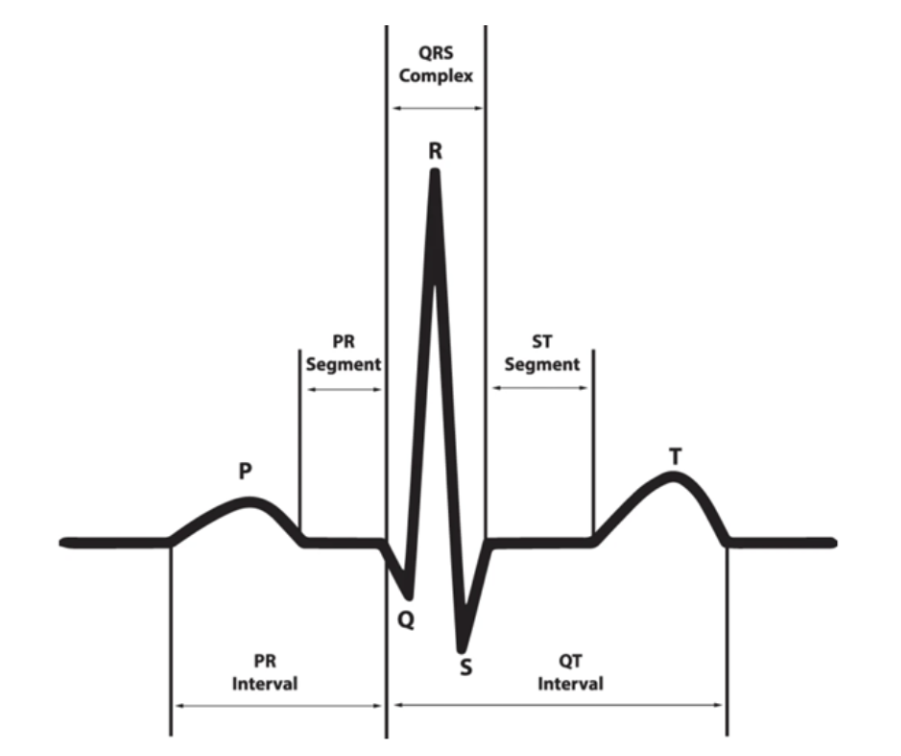
\includegraphics[scale=0.3]{fig1.png}}
% \caption{Example of a figure caption.}
% \label{fig}
% \end{figure}

% Figure Labels: Use 8 point Times New Roman for Figure labels. Use words 
% rather than symbols or abbreviations when writing Figure axis labels to 
% avoid confusing the reader. As an example, write the quantity 
% ``Magnetization'', or ``Magnetization, M'', not just ``M''. If including 
% units in the label, present them within parentheses. Do not label axes only 
% with units. In the example, write ``Magnetization (A/m)'' or ``Magnetization 
% \{A[m(1)]\}'', not just ``A/m''. Do not label axes with a ratio of 
% quantities and units. For example, write ``Temperature (K)'', not 
% ``Temperature/K''.

% \section*{Acknowledgment}

% The preferred spelling of the word ``acknowledgment'' in America is without 
% an ``e'' after the ``g''. Avoid the stilted expression ``one of us (R. B. 
% G.) thanks $\ldots$''. Instead, try ``R. B. G. thanks$\ldots$''. Put sponsor 
% acknowledgments in the unnumbered footnote on the first page.

% \section*{References}

% Please number citations consecutively within brackets \cite{b1}. The 
% sentence punctuation follows the bracket \cite{b2}. Refer simply to the reference 
% number, as in \cite{b3}---do not use ``Ref. \cite{b3}'' or ``reference \cite{b3}'' except at 
% the beginning of a sentence: ``Reference \cite{b3} was the first $\ldots$''

% Number footnotes separately in superscripts. Place the actual footnote at 
% the bottom of the column in which it was cited. Do not put footnotes in the 
% abstract or reference list. Use letters for table footnotes.

% Unless there are six authors or more give all authors' names; do not use 
% ``et al.''. Papers that have not been published, even if they have been 
% submitted for publication, should be cited as ``unpublished'' \cite{b4}. Papers 
% that have been accepted for publication should be cited as ``in press'' \cite{b5}. 
% Capitalize only the first word in a paper title, except for proper nouns and 
% element symbols.

% For papers published in translation journals, please give the English 
% citation first, followed by the original foreign-language citation \cite{b6}.


% \vspace{12pt}
% \color{red}
% IEEE conference templates contain guidance text for composing and formatting conference papers. Please ensure that all template text is removed from your conference paper prior to submission to the conference. Failure to remove the template text from your paper may result in your paper not being published.

\end{document}
